\documentclass[letterpaper,10pt]{article}
\usepackage{ictam}
\usepackage{amsmath,bm}
\usepackage{rotating}
\usepackage{multirow}
\usepackage{caption}
\usepackage{cite}

\begin{document}

\title{A NOVEL STRATEGY FOR COMPACT FINITE DIFFERENCE EVALUATION
ON GPU-ACCELERATED CLUSTERS}

\author[1]{\underline{Ashwin Srinath}}
\author[2]{Daniel Livescu}
\author[3]{Richard S. Miller \footnote{
Corresponding author. Email: rm@clemson.edu}}
\affil[1,3]{
Department of Mechanical Engineering, Clemson University, Clemson, SC 29634-0921}
\affil[2]{Los Alamos National Laboratory, Los Alamos, NM 87544, USA}
\maketitle

\begin{abstract} 
In this work,
we present a novel strategy to solve the
tridiagonal systems arising in such numerical schemes
as compact finite differences
and alternating direction implicit methods
on graphics processing units (GPUs).
We demonstrate the impact of the simple matrix structure
on the \emph{cyclic reduction} algorithm,
and show that precomputation of coefficients appearing in the
algorithm becomes feasible and efficient.
We demonstrate that an implementation using our approach
is able to outperform
the NVIDIA CUSPARSE and multithreaded Intel MKL solvers
on GPU and CPU, respectively.
We apply this tridiagonal solver
to the solution of
compact finite differences on multiple GPUs
distributed in a cluster,
and show scaling for up to 64 GPUs.

\end{abstract}

Compact finite difference schemes
\cite{lele1992compact,kennedy1994several}
are widely used
in computational fluid dynamics (CFD)
for their ability to resolve the high-wavenumber fluctuations
associated with turbulent flows.
In CFD codes using compact schemes,
this generally constitutes a significant portion of the runtime.
The high computational cost associated with
compact finite difference schemes arises from the fact that they require
the solution of tridiagonal linear systems.
Classically, the Thomas algorithm has been used to solve such linear systems.
But with multi-core CPUs, graphics processing units (GPUs),
and more recently,
architectures such as the
Intel Many Integrated Core (MICs)
expected to be mainstays in scientific computing,
such sequential algorithms need to be
replaced by algorithms more suited to these architectures.
In this study,
we develop an algorithm to solve the tridiagonal systems
arising in compact finite difference evaluation
and similar numerical schemes.
Our approach is based on \emph{cyclic reduction},
an extremely successful algorithm for solving multiple
tridiagonal systems on GPUs.
Our work fills two existing gaps in the literature.
First,
whereas current efforts to develop tridiagonal solvers
are focused on single GPUs (e.g., 
\cite{GoSt11CR,
davidson2011register,
esfahanian2014efficient,
tutkun2012gpu,
zhao2015efficiently})
we develop an approach for \emph{multiple} GPUs
in a distributed system (GPU-accelerated clusters).
Second, we specialize the cyclic reduction for the case
of \emph{near-Toeplitz} tridiagonal systems,
a special class of systems arising in numerical schemes
such as compact finite differences,
alternating direction implicit methods,
line relaxation methods, and others.

If $f_i$ represents the value of
a uniformly sampled function with spacing $dx$,
evaluated at the $i^{th}$ sample point,
the first derivative $f^{\prime}_i$ can be approximated from
a relation of the form:
%
\begin{equation}
\begin{split}
    f_i^{\prime} + \
    \alpha(f^{\prime}_{i-1} + f^{\prime}_{i+1})
    = 
    a\frac{f_{i+1} - f_{i-1}}{dx} + \
    b\frac{f_{i+2} - f_{i-2}}{dx} + \
    c\frac{f_{i+3} - f_{i-3}}{dx} + \
    \hdots
\end{split}
\label{eqn:general-compact}
\end{equation}
%
The derivative is defined implicitly,
requiring the solution of a linear system to solve for
the derivative at all points $i$ simultaneously.
An example of such a scheme is the fourth-order accurate
Pad\'{e} scheme, which yields the following system:
%
\begin{equation}
 \label{eqn:compact-tridiagonal-system}
 \begin{bmatrix}
     1&2\\
     1/4&1&1/4\\
     &&\ddots\\
     &&&\ddots\\
     &&&&\ddots\\
     &&&&2&1
  \end{bmatrix}
  \begin{bmatrix}
      f^{\prime}_1 \\
      f^{\prime}_2 \\
      \vdots \\
      \vdots \\
      f^{\prime}_{n-1} \\
      f^{\prime}_n
   \end{bmatrix}
 =
 \begin{bmatrix}
     \frac{-5f_1 + 4f_2 + f_3}{2dx}\\
     \frac{3(f_{3} - f_{1})}{4dx}\\
     \vdots\\
     \vdots\\
     \frac{3(f_{n} - f_{n-2})}{4dx}\\
     \frac{5f_{n} - 4f_{n-1} - f_{n-2}}{2dx}
  \end{bmatrix}
\end{equation}
%
We note the \emph{near-Toeplitz} nature of the tridiagonal system,
i.e., constant diagonal coefficients except near the boundaries.
The cyclic reduction algorithm consists of two phases,
each containing $log_2(N)-1$ steps.
At each step of the \emph{forward reduction} phase,
the odd-indexed equations are eliminated, yielding eventually
a 2-by-2 system.
At each step of the \emph{backward substitution} phase,
the odd-indexed equations are solved from the known solutions
of the even-indexed equations.
Cyclic reduction is well-suited to highly threaded processors
such as GPUs \cite{Zhang2010FTS},
as the individual equations can be processed in parallel.
\pagebreak

When cyclic reduction is applied to
\emph{near-Toeplitz} tridiagonal systems,
we make the important observation that
each forward reduction step preserves the near-Toeplitz
nature of the linear system, i.e.,
the elimination of the odd-indexed equations at each step
yields a new linear system that has
exactly the same near-Toeplitz structure.
This makes it feasible to precompute and store
the coefficients of each linear system,
significantly reducing the amount of computation required.
As it turns out,
this approach also ameliorates several
GPU architecture-specific issues relating to
memory access patterns.
To extend the above approach to multiple GPUs,
we adapt the algorithm described by Mattor et. al
\cite{mattor1995algorithm}
to GPUs.
Our implementation ensures that
each step of this algorithm is performed on the GPU,
avoiding memory transfers to and from the CPU entirely.
%
\begin{figure}
\centering
\begin{minipage}[b]{0.45\textwidth}
\begin{center}
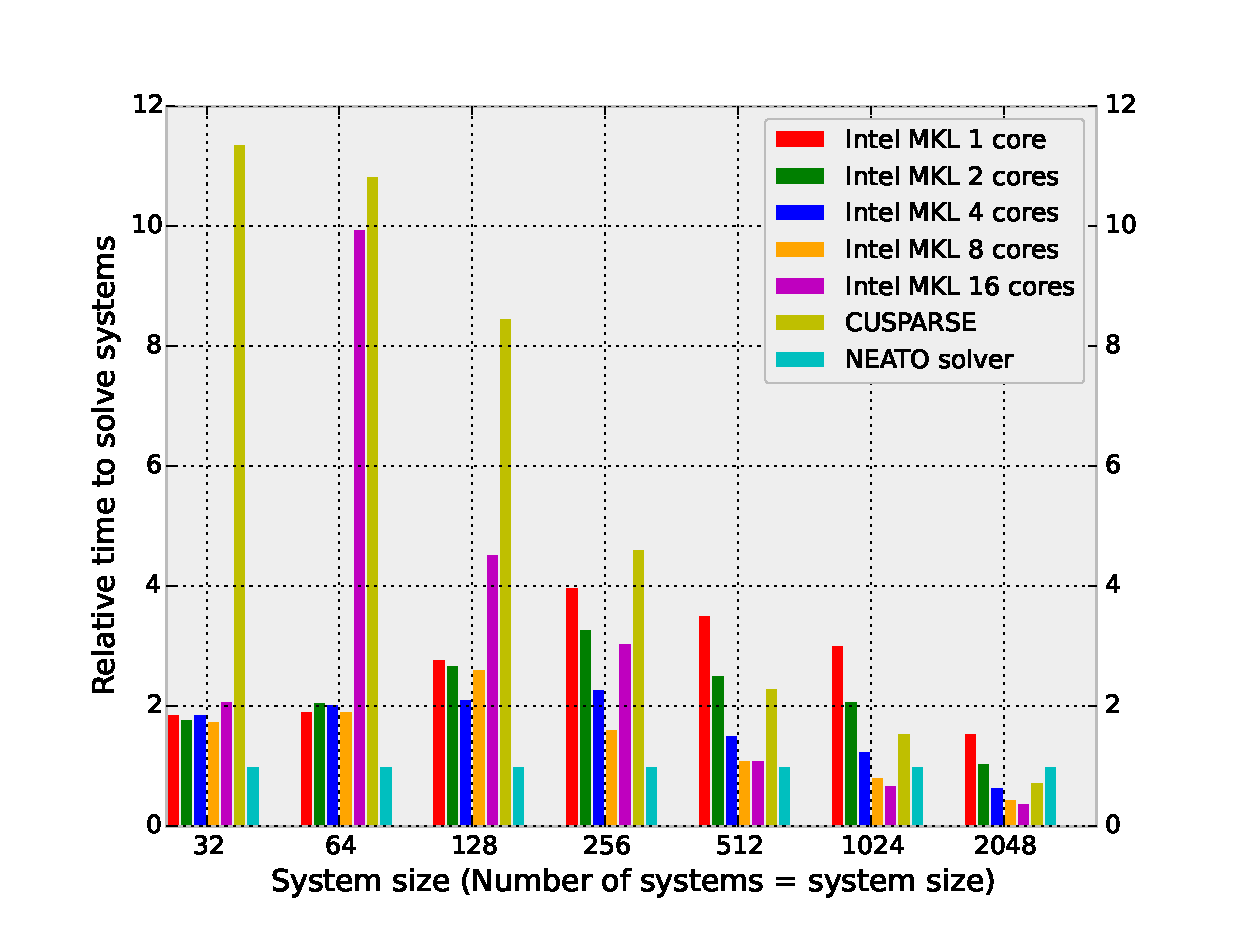
\includegraphics[width=220pt]{fig/bench-2d.eps}
\end{center}
\end{minipage}
\begin{minipage}[b]{0.45\textwidth}
\begin{center}
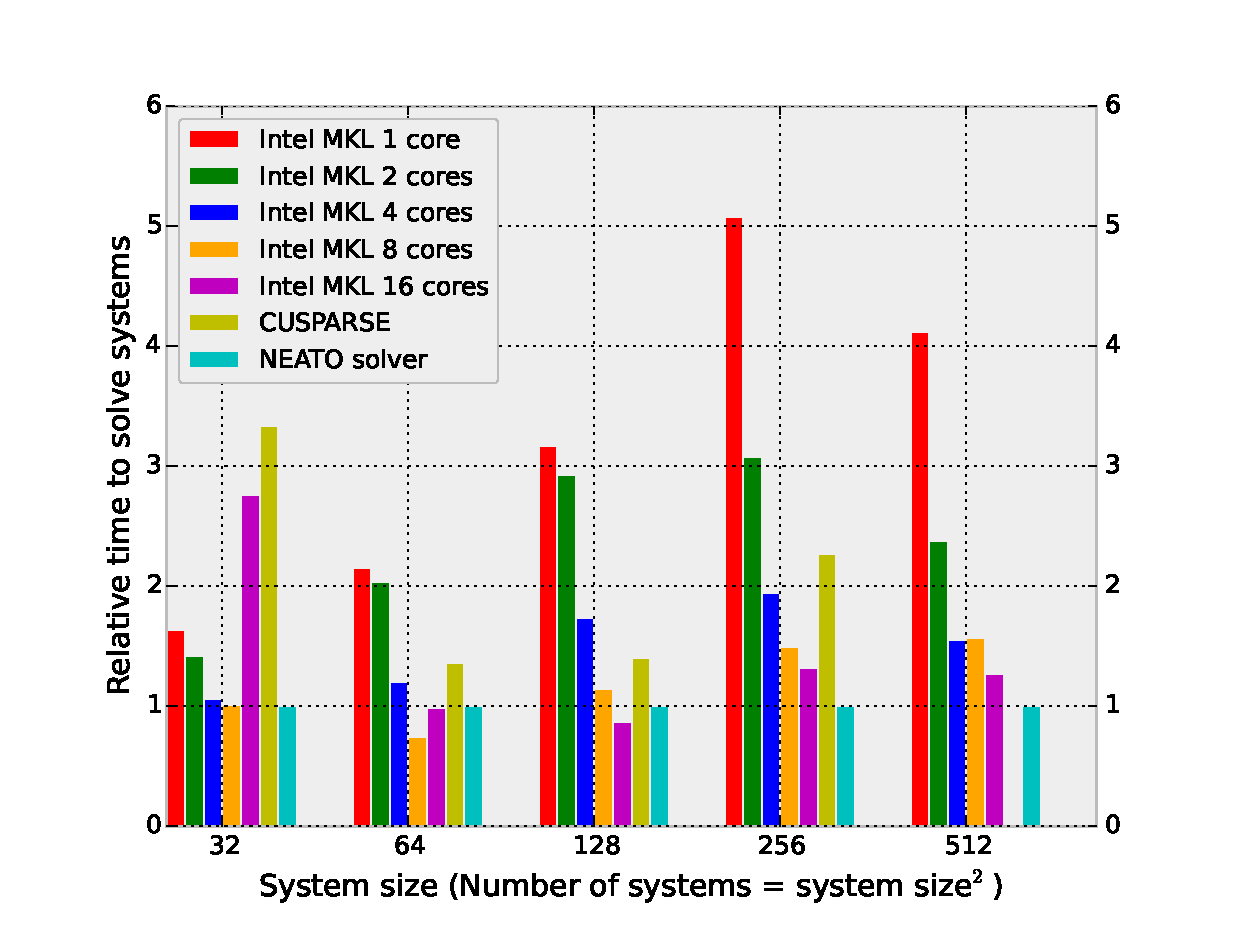
\includegraphics[width=220pt]{fig/bench-3d.eps}
\end{center}
\end{minipage}
\caption{Relative solver performance
for 2-D (left) and 3-D (right) problems.
Relative solver time defined as:}
Time taken by solver/Time taken by NEATO solver
\label{fig:bench}
\end{figure}
%
\iffalse
\begin{figure}
\centering
\begin{minipage}[b]{0.45\textwidth}
\begin{center}
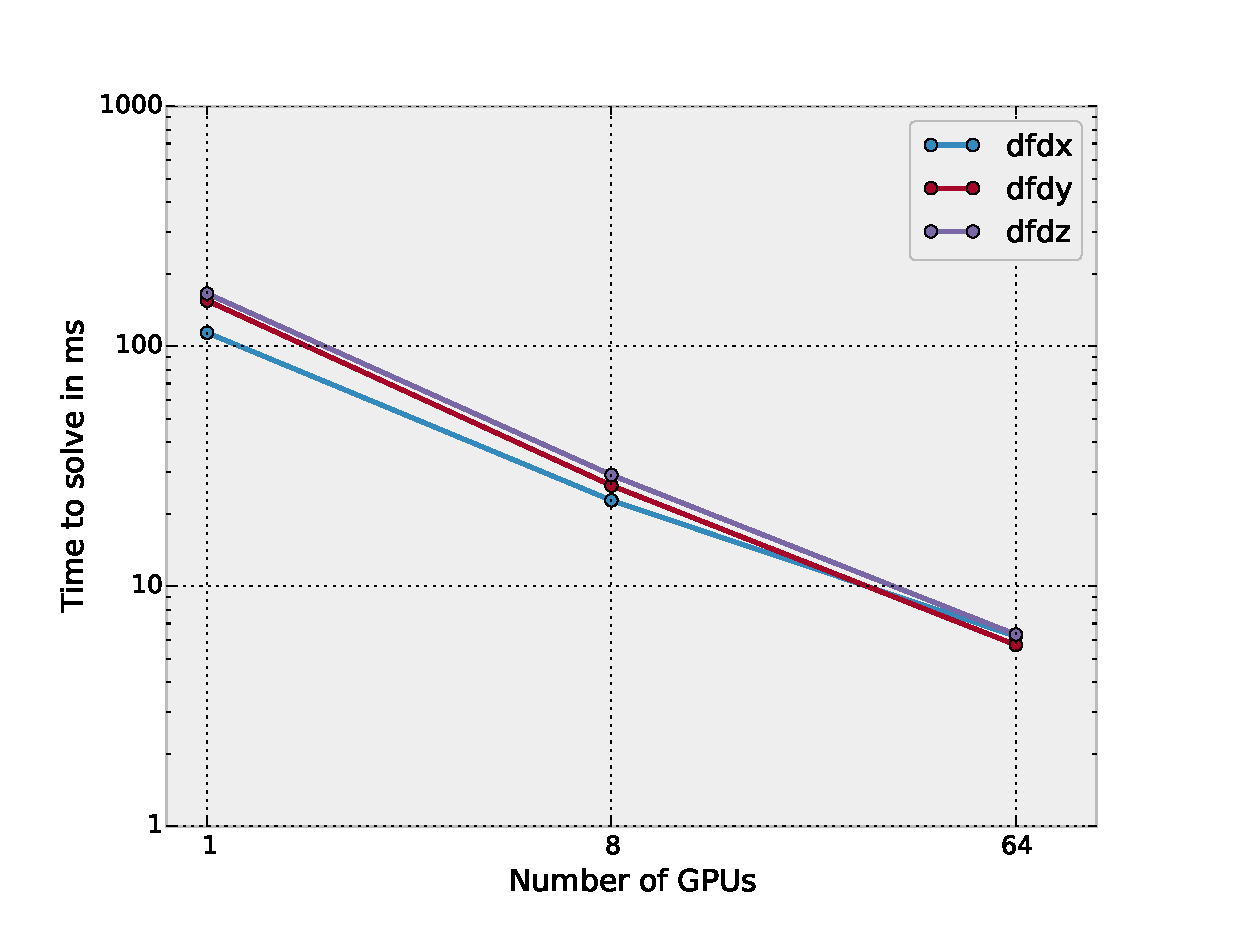
\includegraphics[width=220pt]{fig/strong-scaling-512.eps}
\end{center}
\end{minipage}
\begin{minipage}[b]{0.45\textwidth}
\begin{center}
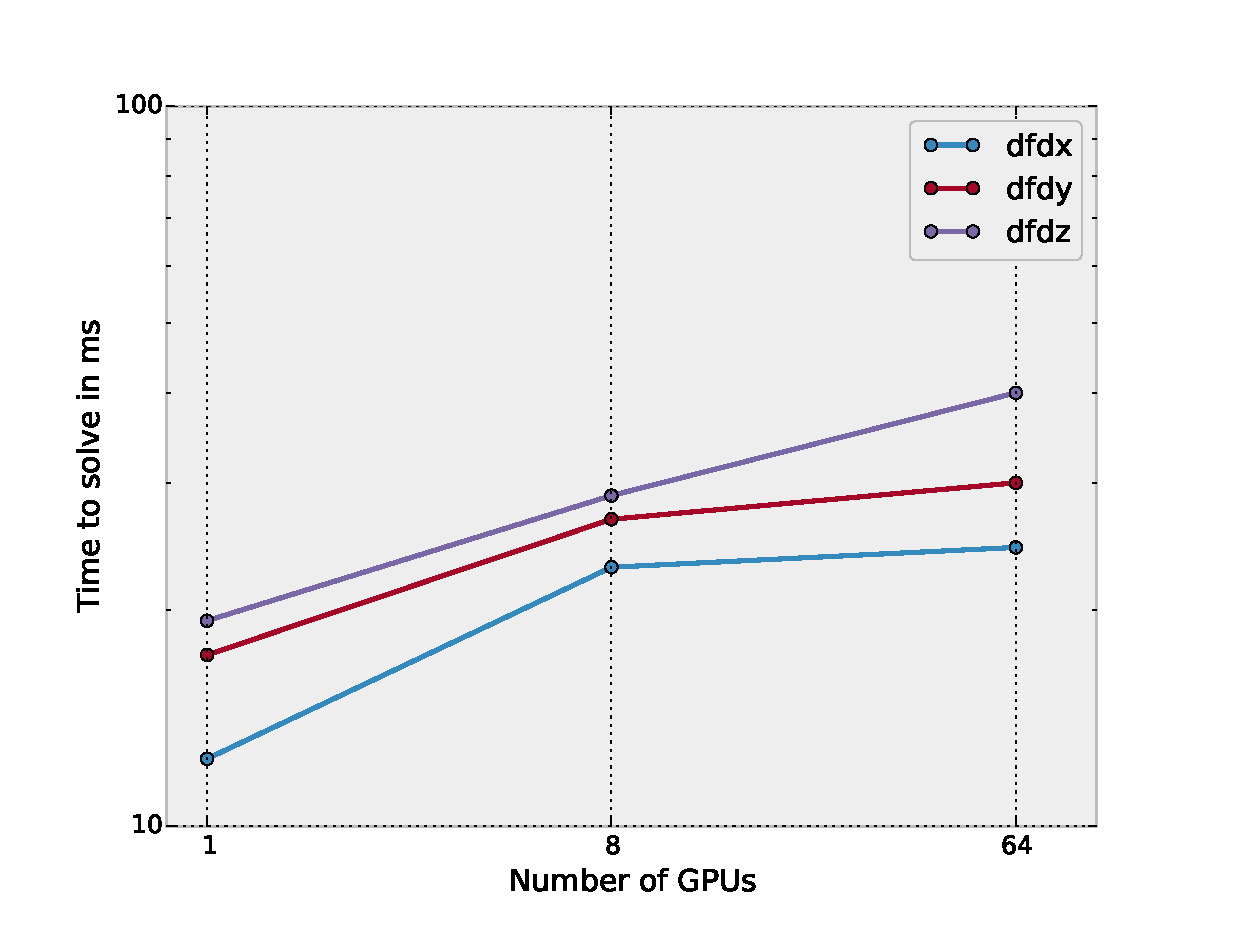
\includegraphics[width=220pt]{fig/weak-scaling-256.eps}
\end{center}
\end{minipage}
\caption{Strong scaling (left) and weak scaling (right)
    for compact finite difference application.
    Problem sizes $512^3$ and $2048^3$ respectively.}
\label{fig:scaling}
\end{figure}
\fi
%
In Fig. \ref{fig:bench},
we compare the performance of our GPU tridiagonal solver
for near-Toeplitz systems (NEATO),
with the equivalent library solvers from
Intel MKL (CPU) and NVIDIA CUSPARSE (GPU).
Here we solve the tridiagonal system in
Eq. (\ref{eqn:compact-tridiagonal-system})
for sizes $N$ and multiple right hand sides $N_{rhs}$.
We present results for two cases, $N_{rhs}=N$,
(representative of 2-D problems)
and $N_{rhs}=N^2$ (3-D problems).
On the GPU, we are consistently able to
obtain better performance than the CUSPARSE solver.
Our GPU solver also outperforms the MKL solver
running on up to 16 CPU cores for large 3-D problems.
We have also investigated the strong and weak scaling for a
multi-GPU compact finite difference application.
Here, we solve for the derivatives of a 3-D function
in a domain distributed among multiple GPUs in a cluster.
We are able to show both strong and weak scaling for up to 64 GPUs
(the largest problem investigated).

\bibliographystyle{unsrt}
\bibliography{bibliography}


\end{document}
